\documentclass[
  lualatex, ja=standard, paper={182mm,257mm}, twocolumn, fontsize=8.5pt, baselineskip=13.5pt,
  line_length=24zw, column_gap=6.1mm, number_of_lines=45, head_space=24.5mm, gutter=0mm
]{jlreq}
\usepackage[haranoaji]{luatexja-preset}
\usepackage{luatexja-fontspec}
\setmainfont{TeX Gyre Termes}
\setsansfont{TeX Gyre Heros}
\usepackage{graphicx}
\usepackage{booktabs}
\usepackage{array}
\usepackage{xurl}
\urlstyle{same}
\usepackage[hidelinks]{hyperref}
\usepackage{fancyhdr}
\usepackage{microtype}
\usepackage{needspace}
\setlength{\parindent}{1\zw}
\setlength{\columnsep}{6.1mm}
\newcommand{\tablefont}{\fontsize{7.5pt}{10.5pt}\selectfont}
\renewcommand{\floatpagefraction}{0.7}
\renewcommand{\topfraction}{0.9}
\pagestyle{fancy}
\fancyhf{}
\renewcommand{\headrulewidth}{0pt}
\fancyfoot[L]{\fontsize{7.5pt}{9pt}\selectfont 教育情報分析研究会\hspace{1em}生成AI論文\hspace{1em}2026}
\fancyfoot[R]{\fontsize{9pt}{11pt}\selectfont\thepage}
\fancypagestyle{plain}{\fancyhf{}\renewcommand{\headrulewidth}{0pt}%
  \fancyfoot[L]{\fontsize{7.5pt}{9pt}\selectfont 教育情報分析研究会\hspace{1em}生成AI論文\hspace{1em}2026}\fancyfoot[R]{\fontsize{9pt}{11pt}\selectfont\thepage}}
\newcommand{\chap}[2]{\par\vspace{13.5pt}\needspace{4\baselineskip}{\centering\gtfamily\bfseries #1．#2\par}\nopagebreak}
\newcommand{\secn}[3]{\par\needspace{3\baselineskip}{\noindent\gtfamily\bfseries #1.#2.\hspace{1\zw}#3\par}\nopagebreak}
\newcommand{\chapspaced}[1]{\par\vspace{13.5pt}\needspace{4\baselineskip}{\centering\gtfamily\bfseries #1\par}\nopagebreak}

\begin{document}
\twocolumn[{%
\noindent\fbox{\parbox[c][16pt][c]{62mm}{\centering\gtfamily\fontsize{9pt}{16pt}\selectfont 生成AI論文}}\hfill{\fontsize{8pt}{12pt}\selectfont 教育情報分析研究会\hspace{1em}生成AI論文\hspace{1em}2026}\par
\vspace{14pt}{\centering\gtfamily\bfseries\fontsize{13pt}{20pt}\selectfont 分数の指導法は理解を高めるか：メタ分析\textsuperscript{†}\par}\vspace{10pt}
{\raggedleft\gtfamily\bfseries\fontsize{10pt}{15pt}\selectfont 教育情報分析研究会\hspace{4mm}\par}\vspace{10pt}
\begin{center}\parbox{\dimexpr\textwidth-12mm\relax}{\setlength{\parindent}{1\zw}分数は数学学習における根強い難点であり，その理解を促す指導法の特定は初等・中等教育の教師にとって重要である．国内外のオープンアクセス論文から条件に合う10本 (参加者687人) を自動で選別・抽出し，数値を本文と照合したうえでランダム効果モデルにより統合した．統合値は \textit{g} = 0.92，95\%信頼区間 [0.50, 1.35]，\textit{I}² = 84.5\% であった．標的を絞った分数指導は１〜９年生の分数理解を有意に改善しうるが，研究間の異質性には慎重な解釈を要する．\par
{\gtfamily キーワード}：メタ分析，分数指導，数学教育，小学校，中学校，指導的介入\par}\end{center}\vspace{4pt}
}]
\footnotetext[0]{\fontsize{7.5pt}{11pt}\selectfont 2026年9月29日公開}
\renewcommand{\thefootnote}{†}\footnotetext{\fontsize{7.5pt}{11pt}\selectfont Society for Educational Data Analysis (SEDA)：Effects of Fraction Instruction Interventions on Students' Fraction Understanding: A Meta-Analysis}
\chap{1}{はじめに}
分数は初等・中等教育の数学において概念的に最も難解な単元の一つとして広く認識されており，これらの学年段階における分数理解の困難は，後の代数などの高度な数学的内容における困難と関連することが多い．１〜９年生は，分数の正式な指導が導入され定着する時期にあたるため，分数の概念的・手続き的理解を支える指導実践を特定する上で重要な時期である．

分数の概念や演算を対象とした様々な指導的介入や教授法が考案されており，技術 (テクノロジー) を活用した教具から，表現に基づく指導系列，誤り分析に基づく指導や言語統合型の指導まで多岐にわたる．採用された研究では，動的なデジタル表現を用いた介入 (BULUT \textit{et al.} 2016)，ストーリーテリングに基づく指導 (LEMONIDIS and KAIAFA 2019)，多重表現指導 (MAHAMA and KYEREMEH 2022，PAL 2014，UBAH 2021)，大小関係の誤概念に対応する反証テキスト (refutation text)  (VAN HOOF \textit{et al.} 2021)，低学力学習者向けの言語・数学統合型スキャフォールディング (PREDIGER and WESSEL 2013)，ゲーミフィケーションを用いた指導 (KARAMERT and VARDAR 2021)，ウェブツールによるワークアウトエグザンプル (worked-out examples) の提示 (TAHIROĞLU and ÖZCAN 2025)，誤りに基づく活動 (SANCAR and ÖZKAYA 2024)などの介入が検討されていた．これらの介入は，通常授業，代替的な教授法，または無処置対照群と比較されることが多く，分数の知識または数学の学力テストが結果指標として用いられていた．

個々の研究は特定の文脈における特定の介入について貴重な知見を提供するが，アプローチ，標本，測定指標の多様性により，単一の研究から分数指導介入の全体的な効果について一般的な結論を導くことは難しい．研究間の効果量を統合する量的統合は，全体的な効果についてより精緻で一般化可能な推定を提供するとともに，学校段階間の変動の検討や統合結果の頑健性の評価を可能にする．

したがって，本メタ分析の目的は，１〜９年生における児童生徒の分数理解に対する分数指導介入の効果に関する量的な実証研究を統合することであった．具体的には，本研究は以下の研究課題に取り組んだ．すなわち，分数指導介入が分数理解に及ぼす全体的な効果はどの程度か，またこの効果は小学生と中学生の間で異なるか，である．

\chap{2}{方法}
\secn{2}{1}{文献の検索}
2026年９月29日に，公開されている２つの書誌データベースを検索した．OpenAlex では題名と要旨を対象に次の検索式を用いた：「(fraction OR fractions) AND (intervention OR instruction OR teaching OR training) AND (elementary OR primary OR “middle school” OR “junior high” OR “lower secondary” OR grade OR children OR pupils)」．対象は2012年以降に刊行されたオープンアクセスの学術誌論文で，分野が教育学 (Education) または発達・教育心理学 (Developmental and Educational Psychology) に分類されたものに限った．国内の研究を含めるため，J-STAGE でも要旨を対象に「分数 指導 小学校」，「分数 授業 効果」のキーワードで検索した (2012年以降)．

\secn{2}{2}{適格基準}
次の条件をすべて満たす研究を対象とした：(a) 対象者：１〜９年生 (小学校・中学校) の児童生徒 (６〜15歳程度)．幼児のみ，高校生のみ，大学生，成人，教員・教員志望者の標本は除く；(b) 扱う要因：分数の概念または演算を対象とした指導的介入または教授法；(c) 比較の対象：通常授業，代替的な教授法，または無処置対照群；(d) 成果指標：分数の知識テストまたは数学の学力テスト；(e) 標準化平均差を計算できる統計量を報告していること．レビュー，質的研究，一事例実験，比較群のない前後比較のみの研究は除外した．

\secn{2}{3}{選別とデータの抽出}
選別とデータの抽出は自動で行った．大規模言語モデル (claude-sonnet-5) が，各論文の題名と要旨を適格基準に照らして評価した．評価の高い論文から本文 (PDF) を取得してテキストに変換し，同じモデルが研究の特徴と要約統計量を抽出した．抽出したすべての数値は，本文にその数字が実際に書かれているかをプログラムで照合し，１つでも見つからない研究は統合から除外した．選別と抽出を人が確認する工程はない．条件を満たす研究が10本を超えた場合は，評価の高い10本を用いた．

\secn{2}{4}{効果量}
標準化平均差として Hedges の g を求めた (HEDGES 1981)．事後テストの平均・標準偏差・人数から計算し，それらが報告されていない場合は独立な２群の t 値，分子の自由度が１の F 値，報告された d または g の順に用いた．正の値は介入群の得点が高いことを表す．１研究につき１つの効果量を用いた．

\secn{2}{5}{統計解析}
効果量はランダム効果モデルで統合し，研究間分散 (\textit{τ}²) は DerSimonian–Laird 法で推定した (DERSIMONIAN and LAIRD 1986)．統合値の信頼区間と検定には，研究数が少ない場合に推奨される Hartung–Knapp–Sidik–Jonkman 法 (HKSJ 法) を用いた (HARTUNG and KNAPP 2001，INTHOUT \textit{et al.} 2014)．異質性は Q，\textit{I}² (HIGGINS and THOMPSON 2002)，\textit{τ}²，95\% 予測区間で評価した．学校段階 (小学校：１〜６年，中学校：７〜９年) ごとに２研究以上ある場合は下位集団分析を行った．頑健性は１研究ずつ除いた分析で確かめ，Egger の回帰検定 (EGGER \textit{et al.} 1997) は研究数が10以上の場合にのみ行うこととした．効果の大きさは慣例的な目安で解釈した (COHEN 1988)．計算は標準的な式 (BORENSTEIN \textit{et al.} 2009) に従い，公開した JavaScript のプログラム (\url{https://github.com/k518-2026/MetaAnalysisToWP}) で行った．

\chap{3}{結果}
\secn{3}{1}{研究の選定}
検索の結果，OpenAlex から150件 (検索式に合う331件のうち上位)，J-STAGE から５件を得た．重複を除くと154件であった．要旨のある145件を選別し，31件を適格の可能性ありと判定した．本文を調べた26件のうち，取得または読み取りができなかったものが11件，適格基準を満たさなかったものが０件，統計量が不足していたものが２件，抽出した数値を本文で確認できなかったものが３件，効果量が現実的でない値になったものが０件であった．最終的に10本の研究をメタ分析に含めた．

\secn{3}{2}{研究の特徴}
対象とした研究 (BULUT \textit{et al.} 2016，KARAMERT and VARDAR 2021，LEMONIDIS and KAIAFA 2019，MAHAMA and KYEREMEH 2022，PAL 2014，PREDIGER and WESSEL 2013，SANCAR and ÖZKAYA 2024，TAHIROĞLU and ÖZCAN 2025，UBAH 2021，VAN HOOF \textit{et al.} 2021) の国，学年，研究デザイン，人数，効果量を表１に示す．参加者は合計687人で，実施国はトルコ，ギリシャ，ガーナ，ベルギー，ドイツ，南アフリカ，インドであった．学校段階別では，小学校 (１〜６年) が８本，中学校 (７〜９年) が２本であった．１研究あたりの人数は40〜120人，研究ごとの効果量は \textit{g} = \ensuremath{-}0.25 から \textit{g} = 1.96 まで分布していた．

\begin{table*}[tb]
\centering
{\tablefont \gtfamily 表１\hspace{1em}対象とした研究の概要\par}\vspace{2pt}
{\tablefont\renewcommand{\arraystretch}{1.12}
\begin{tabular}{>{\raggedright\arraybackslash}p{0.2600\dimexpr\textwidth-12\tabcolsep\relax}>{\raggedright\arraybackslash}p{0.1100\dimexpr\textwidth-12\tabcolsep\relax}>{\raggedright\arraybackslash}p{0.1200\dimexpr\textwidth-12\tabcolsep\relax}>{\raggedright\arraybackslash}p{0.2300\dimexpr\textwidth-12\tabcolsep\relax}>{\raggedright\arraybackslash}p{0.0700\dimexpr\textwidth-12\tabcolsep\relax}>{\raggedright\arraybackslash}p{0.2100\dimexpr\textwidth-12\tabcolsep\relax}}
\toprule
研究 & 国 & 学年 & デザイン & \textit{N} & \textit{g} [95\% CI] \\
\midrule
BULUT \textit{et al.} (2016) & トルコ & 小学3年 & 準実験 & 40 & 0.83 [0.20, 1.47] \\
LEMONIDIS and KAIAFA (2019) & ギリシャ & 小学3年 & 準実験 & 76 & 0.57 [0.12, 1.03] \\
MAHAMA and KYEREMEH (2022) & ガーナ & 小学6年 & 準実験(非同等対照群デザイン) & 96 & 1.39 [0.94, 1.83] \\
VAN HOOF \textit{et al.} (2021) & ベルギー & 小学4年 & ランダム化比較実験 & 76 & \ensuremath{-}0.25 [\ensuremath{-}0.69, 0.20] \\
PREDIGER and WESSEL (2013) & ドイツ & 中学1年(第7学年) & 準実験(事前事後テスト対照群デザイン) & 72 & 0.86 [0.38, 1.34] \\
UBAH (2021) & 南アフリカ & 小学5年 & 準実験（非同等対照群、事前事後テスト） & 120 & 1.96 [1.53, 2.40] \\
PAL (2014) & インド & 小学4年 & 準実験 & 40 & 1.28 [0.61, 1.95] \\
KARAMERT and VARDAR (2021) & トルコ & 小学5年 & 準実験 & 46 & 0.65 [0.07, 1.24] \\
TAHIROĞLU and ÖZCAN (2025) & トルコ & 小学5年 & 準実験 & 77 & 1.15 [0.67, 1.63] \\
SANCAR and ÖZKAYA (2024) & トルコ & 中学1年(6年生) & 準実験 & 44 & 0.77 [0.16, 1.37] \\
\bottomrule
\end{tabular}\par}
\vspace{2pt}{\tablefont\noindent 注：CI＝信頼区間．g は Hedges の g（正の値は介入群が高い）．学年・デザインは論文の本文から自動で抽出した．\par}
\end{table*}
各研究の介入，比較の条件，成果指標を表２に示す．10本はいずれも，介入群と比較群を事後テストで比べた研究である．

\begin{table*}[tb]
\centering
{\tablefont \gtfamily 表２\hspace{1em}各研究の介入・比較の条件・成果指標\par}\vspace{2pt}
{\tablefont\renewcommand{\arraystretch}{1.12}
\begin{tabular}{>{\raggedright\arraybackslash}p{0.2000\dimexpr\textwidth-8\tabcolsep\relax}>{\raggedright\arraybackslash}p{0.3200\dimexpr\textwidth-8\tabcolsep\relax}>{\raggedright\arraybackslash}p{0.2400\dimexpr\textwidth-8\tabcolsep\relax}>{\raggedright\arraybackslash}p{0.2400\dimexpr\textwidth-8\tabcolsep\relax}}
\toprule
研究 & 介入 & 比較の条件 & 成果指標 \\
\midrule
BULUT \textit{et al.} (2016) & GeoGebraを用いた動的な分数指導活動 & 従来の通常の分数指導法 & 22問から成る分数達成度事後テスト(下位問題含め48問) \\
LEMONIDIS and KAIAFA (2019) & 目標焦点型の教育的物語(ストーリーテリング)を用いた分数指導 & 操作教材(具体物・面積モデル・数直線など)を用いた分数指導 & 10項目からなる分数達成度事後テスト \\
MAHAMA and KYEREMEH (2022) & 複数表現に基づく指導法(紙折り、数直線、記号、言語表現を用いる) & 従来型の講義・討論による指導法 & 共通分数の問題解決テスト(10問、30点満点、事後テスト) \\
VAN HOOF \textit{et al.} (2021) & 分数の大小に関する誤概念を明示的に反駁する反駁文による指導 & 誤概念に言及せず説明のみを行う説明文による指導 & コンピュータ化された分数大小比較テストの正答率 \\
PREDIGER and WESSEL (2013) & レジスター関連付け・プッシュドアウトプット・スキャフォールディングを用いた言語・数学統合型分数指導 & 通常の教科書に基づく分数の復習授業 & 標準化された分数テスト(41項目)の事後得点 \\
UBAH (2021) & 具体物から半具体物、記号表象へと段階的に進む複数表象を用いた学習者中心の分数加法指導（Ben教師） & 教師主導の実演によるより手続き的な分数加法指導（Will教師） & 分数達成度テスト（FAT）事後テストの得点 \\
PAL (2014) & 多重表現を用いた概念的知識の関連づけによる分数指導プログラム & 多重表現を関連づけない従来型の分数指導 & 分数概念に関する事前・事後テスト得点 \\
KARAMERT and VARDAR (2021) & ピラミッド型デザインモデルの要素(進捗マップ、バッジ、アバター)を用いたゲーミフィケーション分数指導 & 同じカリキュラムに基づく通常の非ゲーミフィケーション分数指導 & 研究者作成の24項目分数学力テスト \\
TAHIROĞLU and ÖZCAN (2025) & Nearpodを用いた複数解法によるワークアウト例指導 & Nearpodを用いた教科書活動による通常指導 & 分数達成度テスト(FAT)事後テストスコア \\
SANCAR and ÖZKAYA (2024) & 誤りに基づく活動(EBA)を用いた分数指導(誤答と正答を提示し議論する) & 通常の数学カリキュラムに沿った指導(誤答提示なし) & 教科理解テスト(SCT)による分数達成度の事後テスト \\
\bottomrule
\end{tabular}\par}
\vspace{2pt}{\tablefont\noindent 注：論文の本文から自動で抽出し，要約した．\par}
\end{table*}
\secn{3}{3}{全体の効果}
図１に各研究の効果量と統合値をフォレストプロットで示す．四角は各研究の効果量で，大きさは統合における重みを表す．横線は95\%信頼区間，最下段のひし形は統合値である．10本のうち９本で効果量が正の値であり，９本では95\%信頼区間が０を含まなかった．重みが最も大きかったのは UBAH (2021) (10.5\%) であった．

\begin{figure*}[tb]
\centering
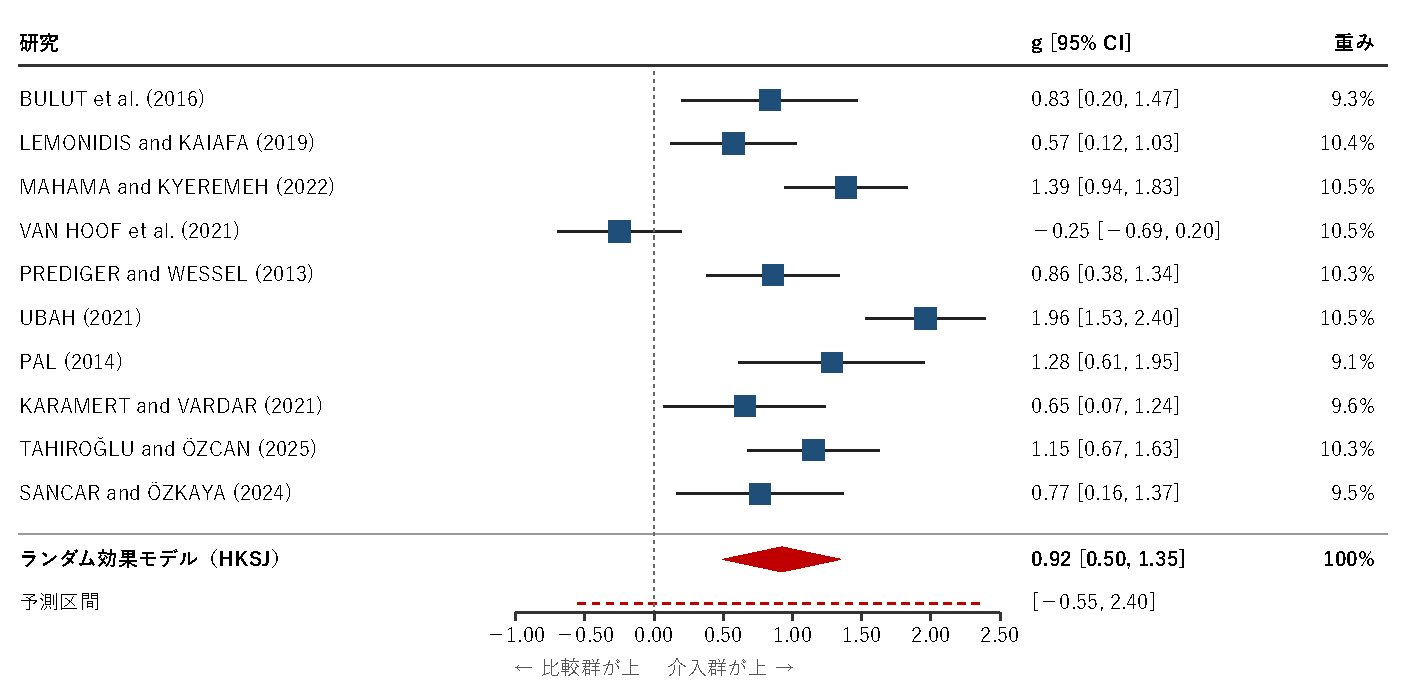
\includegraphics[width=\textwidth]{forest-ja.pdf}\par\vspace{2pt}
{\tablefont\gtfamily 図１\hspace{1em}フォレストプロット\par}{\tablefont 注：四角は各研究の効果量 (大きさは重み)，横線は95\%信頼区間，ひし形は統合値，点線は予測区間を表す．\par}
\end{figure*}
ランダム効果モデルによる統合値は \textit{g} = 0.92，95\% 信頼区間 [0.50, 1.35]，\textit{t}(9) = 4.89，p < .001 であった．慣例的な目安では大きい効果にあたる．固定効果モデルによる推定値は \textit{g} = 0.93 であった．これらの推定値を表３にまとめる．

\secn{3}{4}{異質性}
研究間の異質性は非常に大きかった (\textit{Q}(9) = 58.14，p < .001，\textit{I}² = 84.5\%，\textit{τ}² = 0.364)．95\% 予測区間は \ensuremath{-}0.55 から 2.40 であった．

\secn{3}{5}{下位集団分析と感度分析}
小学校 (１〜６年) では \textit{g} = 0.95，95\% 信頼区間 [0.39, 1.51] (\textit{k} = 8)，中学校 (７〜９年) では \textit{g} = 0.82，95\% 信頼区間 [0.24, 1.40] (\textit{k} = 2) であり，学校段階間の差は統計的に有意ではなかった (\textit{Q}(1) = 0.28，\textit{p} = .598)．１研究ずつ除いた推定値は 0.80 から 1.07 の範囲であった．Egger の検定ではファンネルプロットの非対称性が示されなかった (切片 = \ensuremath{-}1.13，\textit{p} = .846)．下位集団ごとの推定値も表３に示す．

\begin{table*}[tb]
\centering
{\tablefont \gtfamily 表３\hspace{1em}メタ分析の結果\par}\vspace{2pt}
{\tablefont\renewcommand{\arraystretch}{1.12}
\begin{tabular}{lrrrrrrr}
\toprule
モデル & \textit{k} & \textit{N} & \textit{g} & 95\% CI & \textit{p} & \textit{I}² (\%) & \textit{τ}² \\
\midrule
ランダム効果（HKSJ） & 10 & 687 & 0.92 & [0.50, 1.35] & < .001 & 84.5 & 0.364 \\
固定効果 & 10 & 687 & 0.93 & [0.77, 1.09] & < .001 & — & — \\
\hspace{1em}小学校（1〜6年） & 8 & 571 & 0.95 & [0.39, 1.51] & .005 & 87.9 & 0.473 \\
\hspace{1em}中学校（7〜9年） & 2 & 116 & 0.82 & [0.24, 1.40] & .035 & 0.0 & 0.000 \\
\bottomrule
\end{tabular}\par}
\vspace{2pt}{\tablefont\noindent 注：\textit{k}＝研究数．HKSJ＝Hartung–Knapp–Sidik–Jonkman 法による信頼区間．95\% 予測区間 [\ensuremath{-}0.55, 2.40]．\par}
\end{table*}
\chap{4}{考察}
採用された10件の研究にわたる統合効果量は，分数指導介入が児童生徒の分数理解に及ぼす大きな正の効果を示しており，これらの標的介入を受けた児童生徒は，比較条件の児童生徒よりも分数の知識または数学の学力測定において平均的に大きく上回ったことを示している．この効果の大きさは，一般的な教育介入で通常観察される効果よりもかなり大きく，よく設計された分数特化型の指導が，通常授業や代替的な教授法に比べて意味のある利益をもたらす可能性があることを示唆している．

しかし，異質性統計量は研究間の効果量に相当な変動があることを示しており，予測区間は広く，負の値さえ含んでいる．これは，平均的な効果が強く正であるとしても，類似の新たな文脈における特定の介入の効果は，ゼロあるいはわずかに負の値から非常に大きな値まで幅広くありうることを示唆している．この変動は，検討された介入が技術を活用した教具 (BULUT \textit{et al.} 2016，TAHIROĞLU and ÖZCAN 2025)から，表現に基づく指導 (MAHAMA and KYEREMEH 2022，PAL 2014，UBAH 2021)，低学力学習者向けの言語統合型スキャフォールディング (PREDIGER and WESSEL 2013)，ゲーミフィケーション (KARAMERT and VARDAR 2021)，誤りに基づく指導 (SANCAR and ÖZKAYA 2024)まで多岐にわたることに起因する実質的な差異，並びに比較条件，結果指標，標本特性の違いを反映していると考えられる．

小学校段階と中学校段階を比較したサブグループ分析では両群の効果量は同程度であり，サブグループ間差の検定も統計的に有意ではなかった．これは，分数指導介入の効果がいずれかの学校段階に特有のものではなく，これらの学年段階の範囲にわたって一般化しうる可能性を示している．一つずつ除外する感度分析 (leave-one-out) の結果，統合推定値はすべての反復において一貫して大きく正であり，特定の一つの研究が全体の結果を過度に左右していないことが示された．これは，観察された異質性はあるものの，全体的な傾向の頑健性に一定の確信を与えるものである．

注目すべきは，特定の分数の大小関係に関する誤概念を対象とした反証テキスト介入を検討した研究 (VAN HOOF \textit{et al.} 2021)では，比較条件の方が有利となる小さな負の効果が見られた点であり，表現に基づく指導や活動に基づく指導法を用いた研究 (MAHAMA and KYEREMEH 2022，PAL 2014，TAHIROĞLU and ÖZCAN 2025，UBAH 2021)で一般的に見られた強い正の効果とは対照的であった．この対比は，分数に関するすべての指導形態が同等に効果的であるわけではなく，分数の概念に対して能動的で表現豊富，あるいは誤りに着目した取り組みを伴う介入が特に有望である可能性を示唆している．

１〜９年生を担当する教師にとって，これらの知見は，多重表現，能動的な問題解決，技術支援を用いた教具，あるいは標的を絞ったスキャフォールディングを分数指導に取り入れることが，従来の指導のみよりも児童生徒のより強い理解を支える可能性があることを暫定的に示唆している．ただし，研究間の変動を考慮すると，教師や学校管理者は，いかなる単一の手法からも一律の効果が得られると想定するのではなく，具体的な指導法とその文脈を検討すべきである．

\chap{5}{まとめ}
10件の研究を対象とした本メタ分析では，１〜９年生の児童生徒の分数理解に対する分数指導介入の統計的に有意な大きな全体的効果が見出され，小学校段階と中学校段階の間に有意な差はなく，感度分析全体にわたって結果は頑健であった．しかし，研究間の相当な異質性と採用された研究数の少なさから，これらの知見は有望ではあるが予備的な統合として解釈されるべきであり，初等・中等教育全体にわたって分数理解を最も確実に支える具体的な指導上の特徴を明らかにするための，さらなる質の高い研究の必要性が浮かび上がった．

本メタ分析は少数の研究 (\textit{k} = 10) に基づいており，統合推定値の精度と一般化可能性を制限し，特にサブグループ分析と感度分析の統計的検出力を制約している．とりわけ小学校段階と中学校段階の比較は，中学校段階の研究がわずか２件しか含まれていなかった．研究数が少ないことは，統合効果量と異質性の推定値についても慎重な解釈を要することを意味し，これらは今後の研究の追加によって変化しうる可能性がある．

さらに，採用された研究は主に準実験デザインに依拠しており，ランダム化比較試験 (RCT) は１件のみであった．また，結果指標は多様であり，研究者が独自に作成したものが多く，標本も限られた国々から抽出されていたため，統合結果の比較可能性と一般化可能性に影響を及ぼす可能性がある．効果量や研究特性は自動的に抽出されており，本統合には十分に捉えられていない不正確さが含まれる可能性がある．

加えて，本分析は選別とデータ抽出を言語モデルで自動化しており，抽出した数値は本文との文字列の照合でしか確認していない．数値が本文に存在しても，別の群や別の測定の値を取り違えている可能性は残る．対象はオープンアクセスで本文を取得できた論文に限られ，有料の論文や未刊行の研究は含まれていない．

\chapspaced{付\hspace{1\zw}記}
本論文は，教育情報分析研究会が生成AIを用いて自動で作成した「生成AI論文」である．文献の選別，データの抽出，はじめに・考察・まとめの文章の作成には大規模言語モデル (claude-sonnet-5) を用い，統計量はすべてプログラムで計算した．査読は受けていない．

同じ内容の英語版がある (\url{https://raw.githubusercontent.com/k518-2026/MetaAnalysisToWP/main/reports/2026-09-29-math-fraction-instruction/paper-en.pdf})．抽出したデータとプログラムは \url{https://github.com/k518-2026/MetaAnalysisToWP} で公開している．

\chapspaced{参考文献}
{\noindent * はメタ分析に含めた研究を示す．\par}
{\small
\par\noindent\hangindent=2\zw\hangafter=1 BORENSTEIN, M., HEDGES, L. V., HIGGINS, J. P. T. and ROTHSTEIN, H. R. (2009) \textit{Introduction to Meta-Analysis}. Wiley. \url{https://doi.org/10.1002/9780470743386}\par
\par\noindent\hangindent=2\zw\hangafter=1 *BULUT, M., AKÇAKIN, H. Ü., KAYA, G. and AKÇAKIN, V. (2016) The Effects of GeoGebra On Third Grade Primary Students’ Academic Achievement in Fractions. \textit{International Electronic Journal of Mathematics Education}, \textbf{11} (2)：347-255. \url{https://doi.org/10.29333/iejme/338}\par
\par\noindent\hangindent=2\zw\hangafter=1 COHEN, J. (1988) \textit{Statistical Power Analysis for the Behavioral Sciences} (2nd ed.). Lawrence Erlbaum Associates\par
\par\noindent\hangindent=2\zw\hangafter=1 DERSIMONIAN, R. and LAIRD, N. (1986) Meta-analysis in clinical trials. \textit{Controlled Clinical Trials}, \textbf{7} (3)：177-188. \url{https://doi.org/10.1016/0197-2456(86)90046-2}\par
\par\noindent\hangindent=2\zw\hangafter=1 EGGER, M., DAVEY SMITH, G., SCHNEIDER, M. and MINDER, C. (1997) Bias in meta-analysis detected by a simple, graphical test. \textit{BMJ}, \textbf{315} (7109)：629-634. \url{https://doi.org/10.1136/bmj.315.7109.629}\par
\par\noindent\hangindent=2\zw\hangafter=1 HARTUNG, J. and KNAPP, G. (2001) A refined method for the meta-analysis of controlled clinical trials with binary outcome. \textit{Statistics in Medicine}, \textbf{20} (24)：3875-3889. \url{https://doi.org/10.1002/sim.1009}\par
\par\noindent\hangindent=2\zw\hangafter=1 HEDGES, L. V. (1981) Distribution theory for Glass's estimator of effect size and related estimators. \textit{Journal of Educational Statistics}, \textbf{6} (2)：107-128. \url{https://doi.org/10.3102/10769986006002107}\par
\par\noindent\hangindent=2\zw\hangafter=1 HIGGINS, J. P. T. and THOMPSON, S. G. (2002) Quantifying heterogeneity in a meta-analysis. \textit{Statistics in Medicine}, \textbf{21} (11)：1539-1558. \url{https://doi.org/10.1002/sim.1186}\par
\par\noindent\hangindent=2\zw\hangafter=1 INTHOUT, J., IOANNIDIS, J. P. A. and BORM, G. F. (2014) The Hartung-Knapp-Sidik-Jonkman method for random effects meta-analysis is straightforward and considerably outperforms the standard DerSimonian-Laird method. \textit{BMC Medical Research Methodology}, \textbf{14}：25. \url{https://doi.org/10.1186/1471-2288-14-25}\par
\par\noindent\hangindent=2\zw\hangafter=1 *KARAMERT, Ö. and VARDAR, A. K. (2021) The effect of gamification on young mathematics learners’ achievements and attitudes. \textit{Journal of Educational Technology and Online Learning}, \textbf{4} (2)：96-114. \url{https://doi.org/10.31681/jetol.904704}\par
\par\noindent\hangindent=2\zw\hangafter=1 *LEMONIDIS, C. and KAIAFA, I. (2019) The Effect of Using Storytelling Strategy on Students’ Performance in Fractions. \textit{Journal of Education and Learning}, \textbf{8} (2)：165. \url{https://doi.org/10.5539/jel.v8n2p165}\par
\par\noindent\hangindent=2\zw\hangafter=1 *MAHAMA, P. N. and KYEREMEH, P. (2022) Impact of multiple representations-based instruction on basic six pupils’ performance in solving problems on common fractions. \textit{Journal of Mathematics and Science Teacher}, \textbf{3} (1)：em023. \url{https://doi.org/10.29333/mathsciteacher/12610}\par
\par\noindent\hangindent=2\zw\hangafter=1 *PAL, M. (2014) Making Conceptual Knowledge Connections to Clear Misconceptions in Fractions in Primary Classrooms. \textit{IOSR Journal of Research \& Method in Education (IOSRJRME)}, \textbf{4} (2)：12-18. \url{https://doi.org/10.9790/7388-04241218}\par
\par\noindent\hangindent=2\zw\hangafter=1 *PREDIGER, S. and WESSEL, L. (2013) Fostering German-language learners’ constructions of meanings for fractions—design and effects of a language- and mathematics-integrated intervention. \textit{Mathematics Education Research Journal}, \textbf{25} (3)：435-456. \url{https://doi.org/10.1007/s13394-013-0079-2}\par
\par\noindent\hangindent=2\zw\hangafter=1 *SANCAR, E. and ÖZKAYA, M. (2024) Error-based Activity Applications in Sixth Grade Fraction Teaching. \textit{Studia paedagogica}, \textbf{29} (2)：33-65. \url{https://doi.org/10.5817/sp2024-2-2}\par
\par\noindent\hangindent=2\zw\hangafter=1 *TAHIROĞLU, N. G. and ÖZCAN, Z. Ç. (2025) Impact of worked-out examples via a Web 2.0 tool on fifth graders achievement, attitudes, and motivation in mathematics. \textit{Journal of Pedagogical Research}. \url{https://doi.org/10.33902/jpr.202533896}\par
\par\noindent\hangindent=2\zw\hangafter=1 *UBAH, I. J. (2021) The impact of different approaches to the teaching of Grade 5 fraction by three experienced teachers. \textit{South African Journal of Childhood Education}, \textbf{11} (1). \url{https://doi.org/10.4102/sajce.v11i1.854}\par
\par\noindent\hangindent=2\zw\hangafter=1 *VAN HOOF, J., ENGELEN, A.-S. and VAN DOOREN, W. (2021) How robust are learners’ misconceptions of fraction magnitude? An intervention study comparing the use of refutation and expository text. \textit{Educational Psychology}, \textbf{41} (5)：524-543. \url{https://doi.org/10.1080/01443410.2021.1908521}\par
}
\chapspaced{Summary}
{\setlength{\parindent}{1\zw}\noindent Fractions are a persistent stumbling block in mathematics learning, and identifying instructional approaches that improve fraction understanding matters for teachers in primary and lower secondary classrooms. Using an automated workflow in which every extracted number was verified against the full text, 10 open-access studies (\textit{N} = 687) were pooled with a random-effects model. The pooled effect was \textit{g} = 0.92, 95\% CI [0.50, 1.35], with \textit{I}² = 84.5\%. These findings suggest that targeted fraction instruction can meaningfully improve fraction understanding among students in grades 1-9, though heterogeneity across studies warrants cautious interpretation.\par
KEYWORDS: META-ANALYSIS, FRACTION INSTRUCTION, MATHEMATICS EDUCATION, ELEMENTARY SCHOOL, LOWER SECONDARY SCHOOL, INSTRUCTIONAL INTERVENTION\par}
\end{document}
